\chapter{Background}
This project is focused on computer vision for detecting and tracking humans in the surroundings, estimating their trajectories and distance from the PWU, the reactive control systems that prevent collisions with the detected objects as well as the augmented reality display to provide visual cues to the PWU.

\section{Human Detection}
Human detection is a subset of the classic computer vision problem of object detection. In order to develop an augmented reality system that will help PWUs to navigate in public spaces, it is essential for the system to be able to discern humans from the surroundings.

\subsection{Definition of Requirements}
 The problem arises in crowded areas, whereby individuals are occluded by other people or objects in front of them, leaving only certain body parts visible. As such, we began our research with the problem of being able to detect people in images where identifiying parts of the body are not always visible.

\subsection{Review of Existing Methodologies}
A related field of research is that of people counting and human detection in visual surveillance in public areas. Where the problem differs is that surveillance benefits from being able to rely on cameras with a good view of the crowd from above, whereas for a PWU, the camera will not have as high of a vantage point, making detecting every single individual in a crowd impossible. 

Despite the disadvantage, similar techniques can be used to detect humans in video. Most methods can be classified into two categories \cite{Hou2010}. The first technique, foreground detection, attempts to model the background of an image and then detect the changes that occur between frames. The second category involves exhaustively searching the image with a scanning window, and deciding if each window can be classified into a human shape.

\begin{figure}[ht]
	\begin{subfigure}[b]{.5\textwidth}
		\centering
		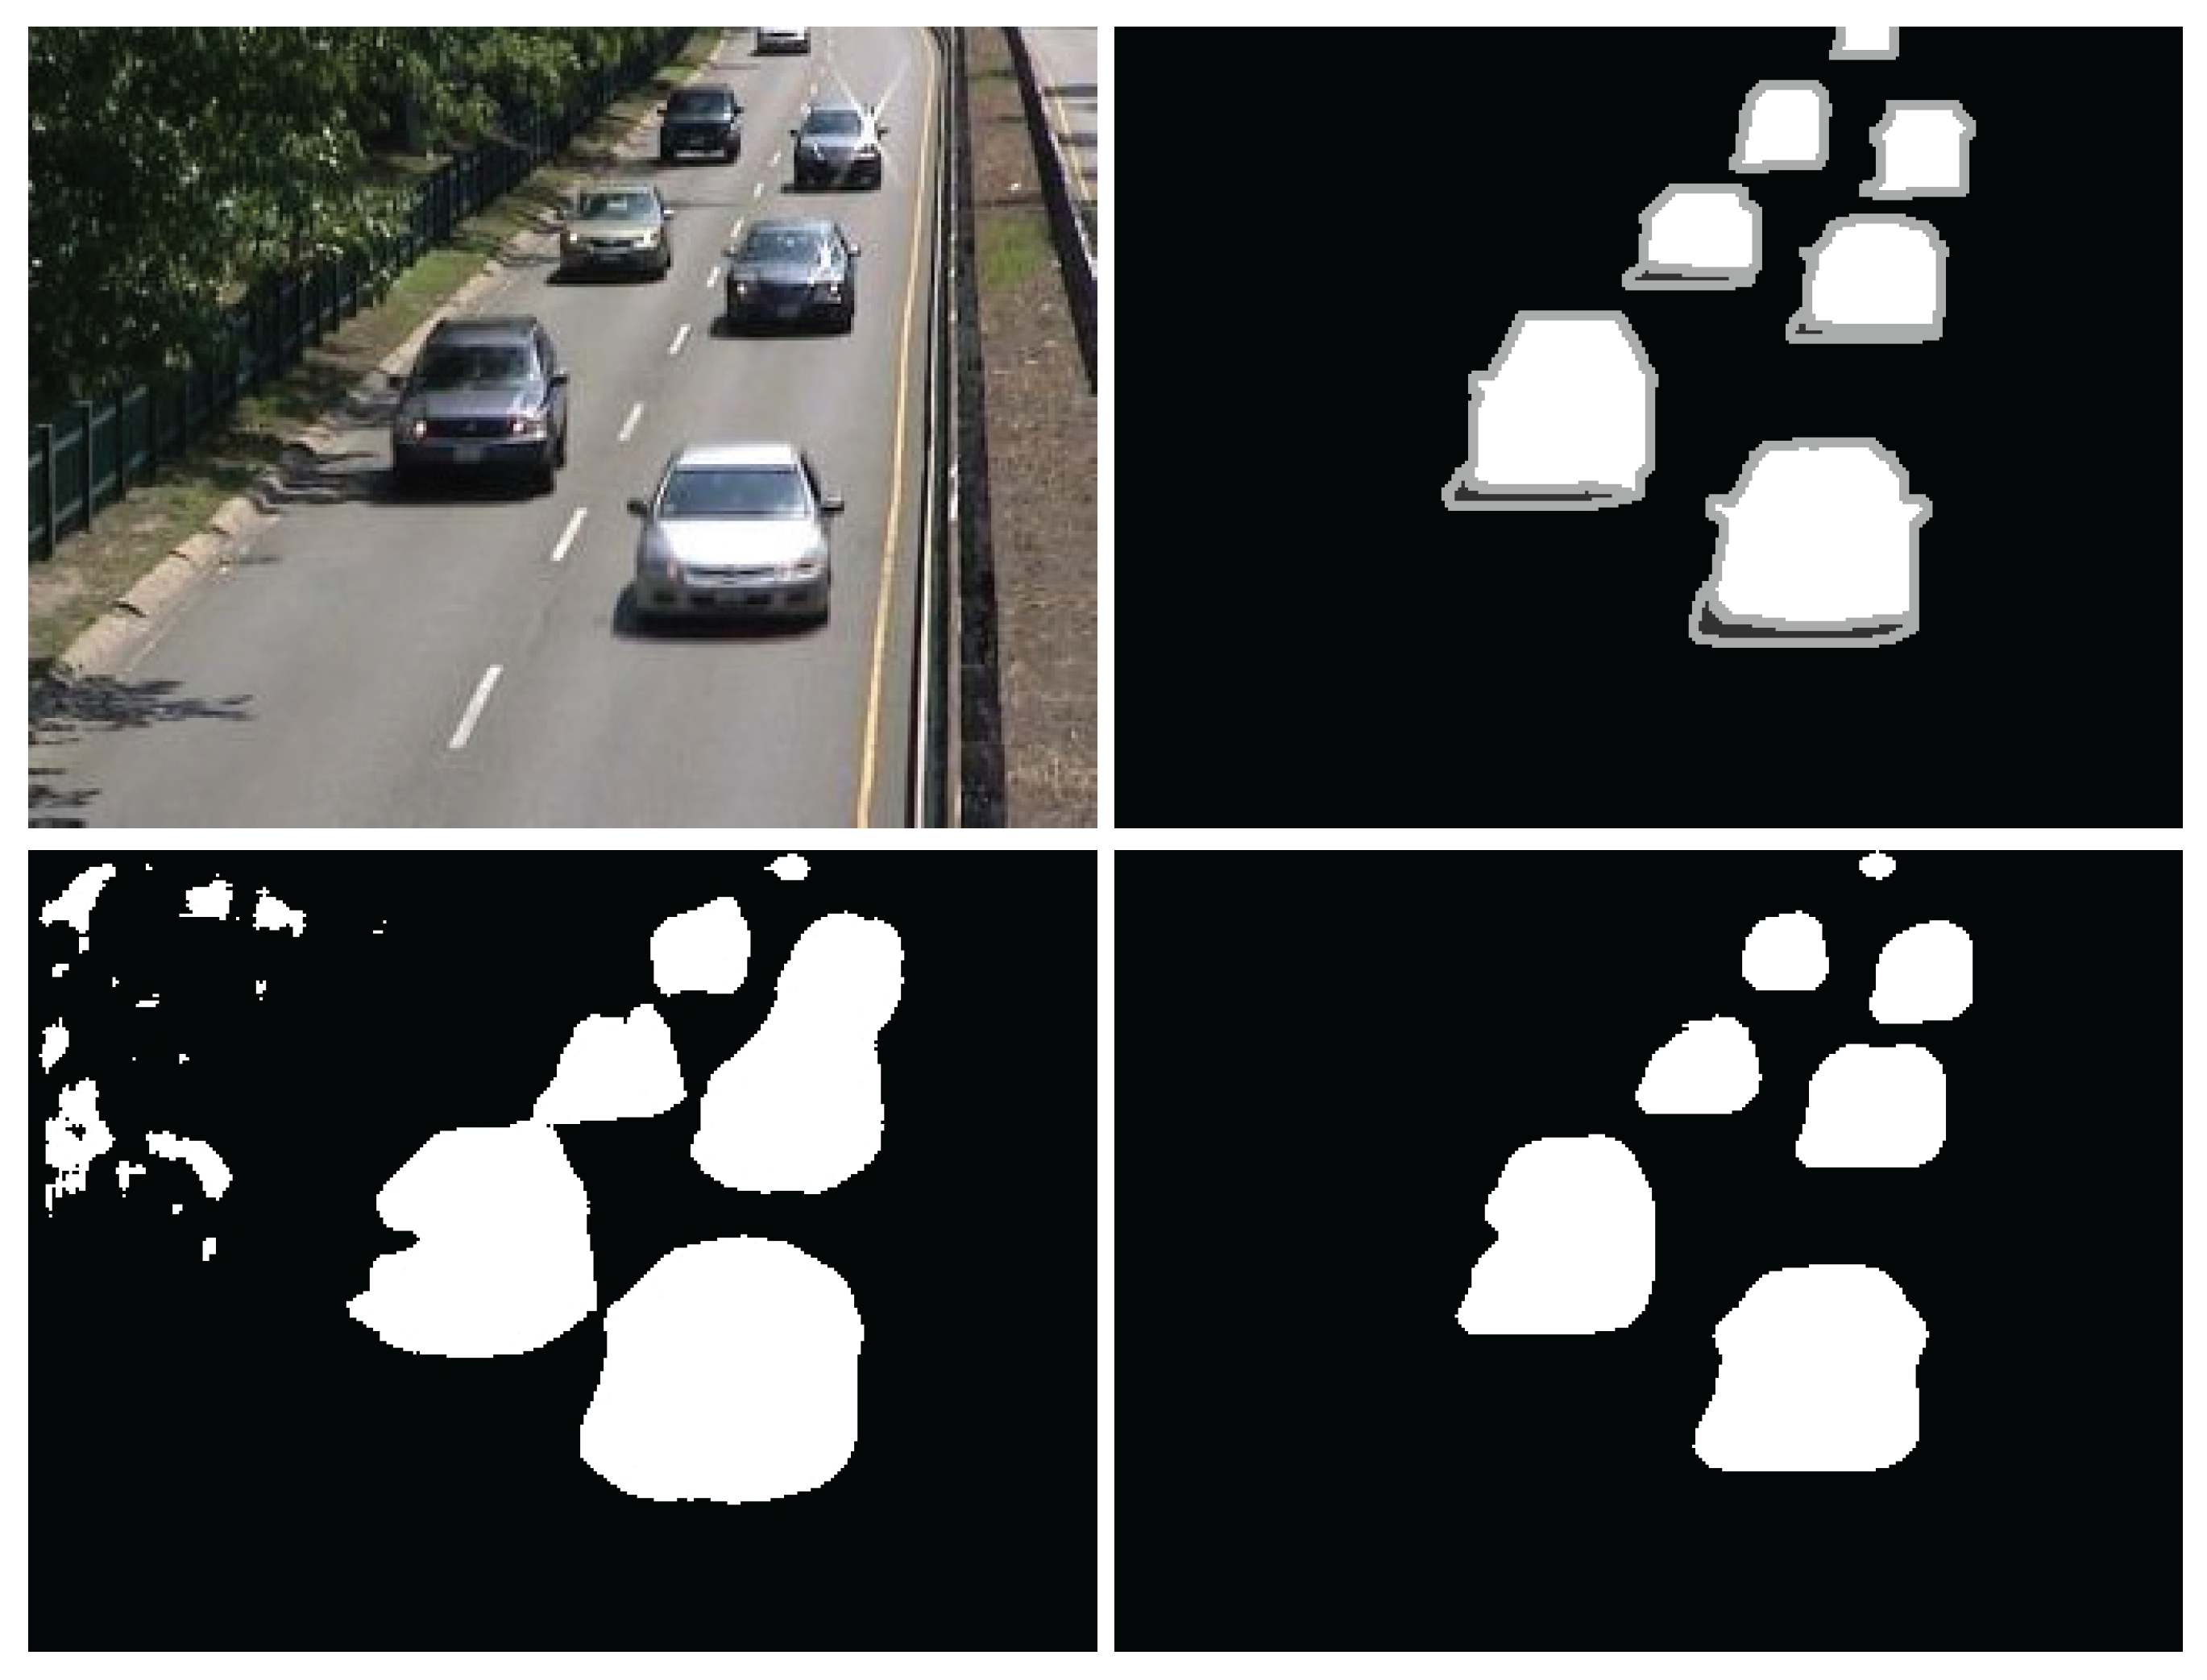
\includegraphics[width=.9\linewidth]{img/chapter2_background/robustBackgroundSubtraction.png}
		\caption{Foreground Detection \cite{Zeng2017}}
	\end{subfigure}%
	\hspace{\fill} 
	\begin{subfigure}[b]{.5\textwidth}
		\centering
		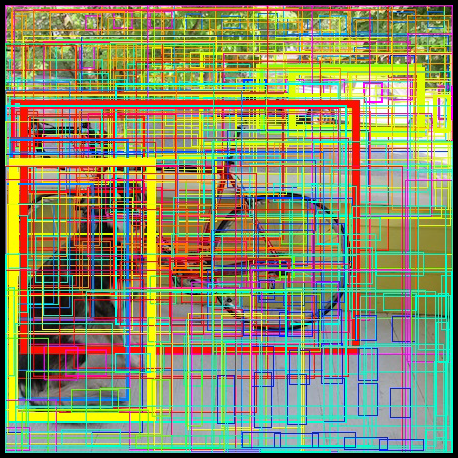
\includegraphics[width=.675\linewidth]{img/chapter2_background/yoloBBBoxes.png}
		\caption{Scanning Window \cite{Redmon}}
	\end{subfigure}
	
	\begin{center}
		\caption{Comparison of Foreground Detection and Scanning Windows}
		\label{fig:HDS_Test_Locations}
	\end{center}
\end{figure}

\subsubsection{Foreground Detection}
Background subtraction is a widely used approach for detecting moving objects \cite{Piccardi2004}. A temporal average filter can be used to find the median of all the pixels in an image to form a reference image. Frames with moving objects can then be compared pixelwise to the reference, and a threshold set to determines if the pixel is part of the background or foreground. People counting and human detection can then be achieved by segmenting the foreground image into individuals.

\paragraph{} However, this technique relies on a static camera in a well placed location. This brings up several reasons as to why this method would not be suitable for this project. Firstly, the camera available is part of a head-mounted augmented reality device. The wearer has the ability to move the camera in 6 degrees of freedom. Secondly, the wearer will also be navigating a powered wheelchair. As a result, the background is constantly changing, and the reference image would require constant recomputation before human detection can even begin.

\subsubsection{Scanning Windows}
Due to the ever-changing surroundings of a mobile robot, a better approach for object detection is to exhaustively search an image using scanning windows and determining if an object was detected in each window. However, it must be noted that this method is computationally expensive. In order to achieve real-time detection on a mobile robot, the use of a graphics processing unit (GPU) should be considered \cite{Hirabayashi}.


% Object Detection
% Traditional methods vs CNN
% Need to be able to detect people in real time
% Need for a GPU for training and runtime

\section{Object Tracking}
% Object tracking
% Track objects across frame to get a sense of direction

\section{Head Pose Estimation}

\section{Body Pose Estimation}
% Human body pose estimation
% The pose of the shoulders and body can be used to determine the direction

\section{SLAM}

\section{Augmented Reality Headsets}